% =============================================================================
% =============================================================================
% =============================================================================
\section{Electron Inertial Effects}
  \label{sec_inertia}

As laid out in \cref{sec_tuna}, Tuna resolves neither parallel currents nor parallel electric fields. This limits the model's applicability to \todo{direct acceleration of particles? double layers? \Alfven{}ic aurorae? } and other topics closely related to field line resonance. 

Parallel currents and electric fields can be added to Tuna through the consideration of electron inertial effects in \ohmlaw:
\begin{align}
  0 &= \sz E_z - J_z & \text{becomes} & & \ddt J_z &= \frac{n e^2}{\me} E_z - \nu J_z
\end{align}

With the addition of the electron inertial term, it is necessary to track the parallel current independent of the parallel electric field\footnote{The parallel current $J_z$ is defined on the same points of the Yee grid as $E_z$. It is offset in time by half of a time step. }. Solving by integrating factors gives
\begin{align}
  J_3 &\assign J_3 \, \exp \arg{ - \nu \dt } + \dt \, \frac{n e^2}{\me} E_3 \, \exp \arg{ -\nu \tfrac{\dt}{2} }
\end{align}

From there, the parallel electric field can be updated directly; \cref{e3_final} is replaced by the following: 
\begin{align}
  E_3 &\assign E_3 + c^2 \dt \, \lr{ g_{31} F^1 + g_{33} F^3 } - \frac{\dt}{\ez} J_3
\end{align}

The present section explores the complications that arise from the addition of the electron inertial term to \ohmlaw, as well as a few results that may be gleaned despite those complications. Notably -- for reasons discussed in \cref{sec_lengths} -- the results presented in \cref{ch_results} do not make use of the electron inertial term. 

% -----------------------------------------------------------------------------
% -----------------------------------------------------------------------------
% -----------------------------------------------------------------------------
\subsection{The Boris Factor}
  \label{sec_boris}

With the addition of the electron inertial term, a cyclical dependence appears between \amplaw and \ohmlaw:
\begin{align}
  \ddt E_z &\sim -\frac{1}{\ez} J_z &
  & \text{and} & 
  \ddt J_z &\sim \frac{n e^2}{\me} E_z &
  & \text{so} &
  \frac{ \partial^2 }{ \partial t^2 } E_z &\sim -\op^2 E_z
\end{align}

That is, electron inertial effects come hand in hand with the plasma oscillation. 

\begin{figure}[!htb]
    \centering
    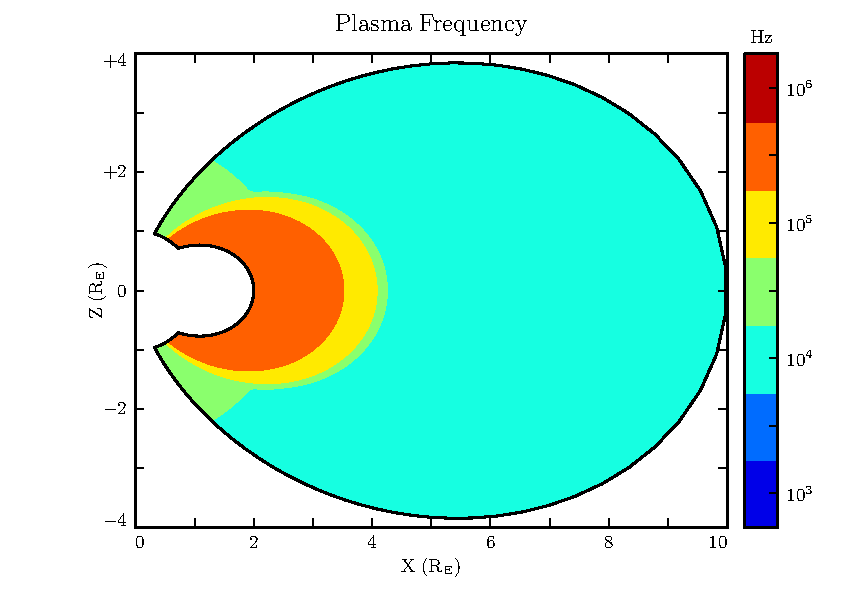
\includegraphics[width=\textwidth]{figures/op.pdf}
    \caption[Plasma Frequency Profile]{
      The plasma frequency reaches a peak value just under \SI{e6}{\Hz} near the equator. Outside the plasmasphere, its value is closer to \SI{e4}{\Hz}, which is still not well-resolved by Tuna's usual time step.  
    }
    \label{fig_op}
\end{figure}

As mentioned in \cref{sec_math} and shown in \cref{fig_op}, plasma oscillation is quite fast -- several orders of magnitude smaller than Tuna's time step as determined in \cref{sec_coords} (\about\SI{10}{\us}). This poses a conundrum. At Tuna's usual time step, the plasma oscillation becomes unstable within seconds\footnote{\todo{The plasma oscillation is unstable at large time steps because of overcorrection. For stability, $\op \dt < 1$ is necessary. }}. On the other hand, reducing the time step by three orders of magnitude to resolve the plasma oscillation is computationally infeasible; a run previously slated for an hour would now require six weeks to complete. 

As it happens, this problem can be solved by artificially increasing the parallel electric constant above its usual value of \ez. Doing so lowers both the speed of light and the plasma frequency within the simulation. 

This technique -- and others like it -- has been widespread in numerical modeling since it was presented by Boris in 1970\cite{boris_1970}. More recently, Lysak and Song considered its use specifically for the case of electron inertial effects\cite{lysak_2001}. The following paraphrases their argument. 

Supposing that the current and electric field are oscillating at frequency $\omega$, the parallel components of \amplaw and \ohmlaw can be written
\begin{align}
  - i \omega \ez E_z &= \oomz F_z - J_z & - i \omega J_z &= \frac{n e^2}{\me} E_z - \nu J_z
\end{align}

Then, eliminating the current, the parallel electric field can be related to the curl of the magnetic field by
\begin{align}
  \label{boris_criterion}
  \lr{ 1 - \frac{\omega^2 - i \nu \omega}{\op^2} } E_z &= \frac{c^2}{\op^2} \lr{ \nu - i \omega } F_z
\end{align}

In \cref{boris_criterion}, $\frac{c}{\op}$ is the electron inertial length. While the speed of light and the plasma frequency each depend on \ez, their ratio does not. This allows an estimation of how much the model should be affected by an artificially-large electric constant (and thus an artificially-small plasma frequency): so long as $\frac{\omega^2 - i \nu \omega}{\op^2}$ remains small compared to unity, the model should behave faithfully. 

For waves with periods of a minute or so, even perhaps-implausibly large Boris factors are allowed; for example, increasing \ez by a factor of \num{e6} gives $\left| \frac{\omega^2 + i \omega \nu}{ \op^2 } \right| \lesssim 0.01$. %In some places, this causes the speed of light to fall below the \Alfven speed; R{\"o}nnmark\cite{ronnmark_2000} terms this behavior ``anisotropic vacuum.''

%\todo{Generalized \ohmlaw, in case we decide we need it. Could talk through why all of the other terms are OK to neglect.  
%\begin{align}
%  \vec{E} + \vec{U} \! \times \! \vec{B} & = 
%  \eta \vec{J} + \tfrac{\me}{n e^2} \lrb{
%    \tfrac{\partial}{\partial t} \vec{J} + \nabla \cdot \lr{ 
%      \vec{J} \, \vec{U} + \vec{U} \,\vec{J} +
%      \tfrac{1}{n e} \vec{J} \, \vec{J} } } +
%  \tfrac{1}{n e} \vec{J} \! \times \! \vec{B} -
%  \tfrac{1}{n e} \div{ \vec{P_e} }
%\end{align}
%}

% -----------------------------------------------------------------------------
% -----------------------------------------------------------------------------
% -----------------------------------------------------------------------------
\subsection{Parallel Currents and Electric Fields}
  \label{sec_inertia_fields}

%\todo{Parallel electric fields, supposedly, only appear at high altitude. \cite{marklund_1997,carlson_1998}. }

%\todo{Integrate up a parallel electric field to see the potential difference. Compare to the relation seen by \cite{olsson_1996}, $J_\parallel \sim \Psi_\parallel$ by a proportionality constant of \SIrange{e-8}{e-10}{\S/\meter\squared}. }

As discussed in \cref{sec_math}, parallel electric fields in this regime are expected to be several orders of magnitude smaller than the perpendicular electric fields. 

\todo{Simulations show this to be the case. Parallel electric fields are large compared to zero, of course, but small compared to the perpendicular electric fields. }

\todo{Even side by side, no difference is apparent in the magnetic fields between runs with and without electron inertial effects. This is what we expect: $\ddt \vec{B} = -\curl{E}$, so the magnetic fields are coupled to the parallel and perpendicular electric fields with equal weight. The parallel electric fields are orders of magnitude smaller, so their effect on the magnetic field is four orders of magnitude less. }

%\begin{figure}[H]
%    \centering
%    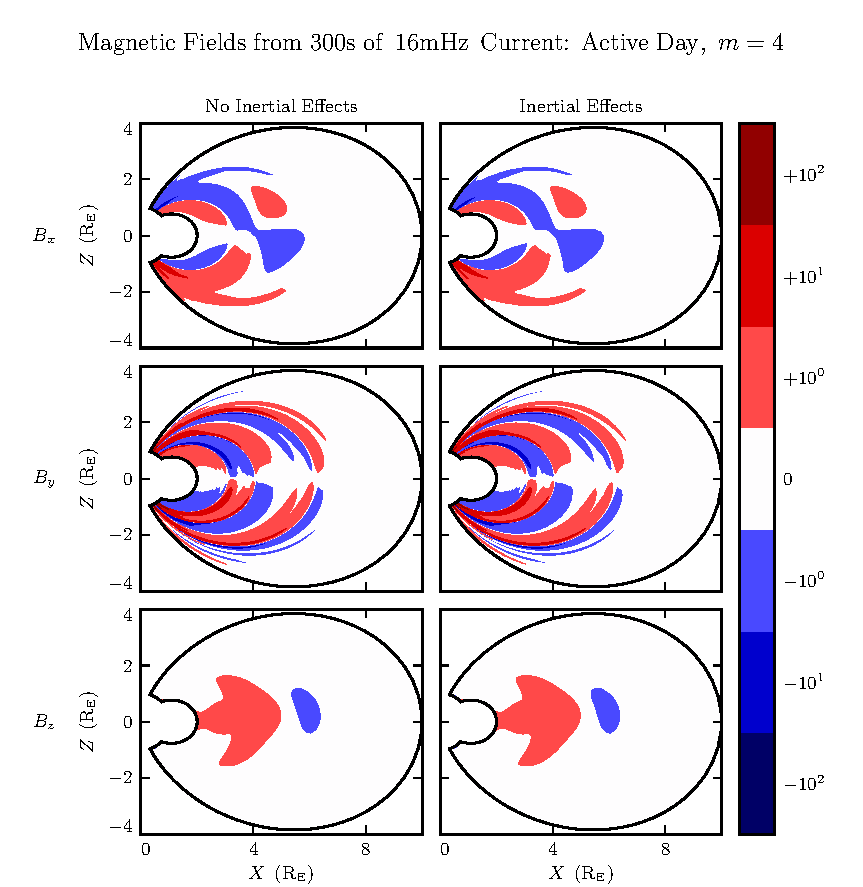
\includegraphics[width=\textwidth]{figures/B_1_004_016mHz.pdf}
%    \caption[Magnetic Fields With and Without Electron Inertia]{
%      The addition of electron inertial effects, with no other changes to the model, does not visible change the output. In a way, this is reassuring, since the alternative is to cast doubt on past work. 
%    }
%    \label{fig_B_1_004_016mHz}
%\end{figure}

\todo{This is good -- it means that we aren't casting doubt on past results, and on the results presented in \cref{ch_results}, which do not use electron inertial effects. }

\begin{figure}[!htb]
    \centering
    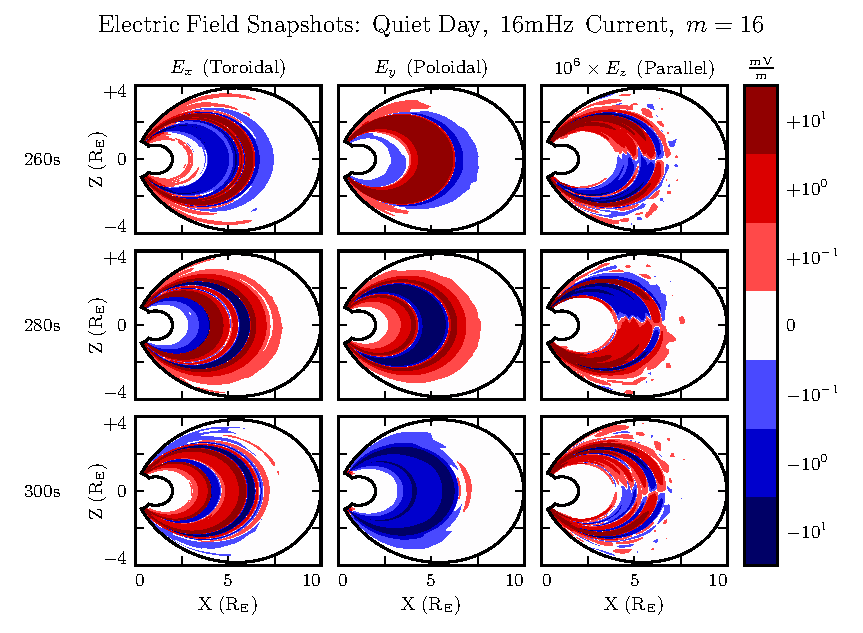
\includegraphics[width=\textwidth]{figures/electric_field_snapshots.pdf}
    \caption[Electric Field Snapshots]{
      Parallel electric fields are smaller than perpendicular electric fields by at least four orders of magnitude. This is a significant increase compared to runs without electron inertial effects (which take parallel electric fields to be uniformly zero), but not enough to appreciably affect $\curl{E}$. 
    }
    \label{fig_electric_field_snapshots}
\end{figure}

\todo{It's interesting to note the structure. Whereas the poloidal and toroidal electric fields have an antinode at the equator, the parallel electric field has an antinode. }




\begin{figure}[!htb]
    \centering
    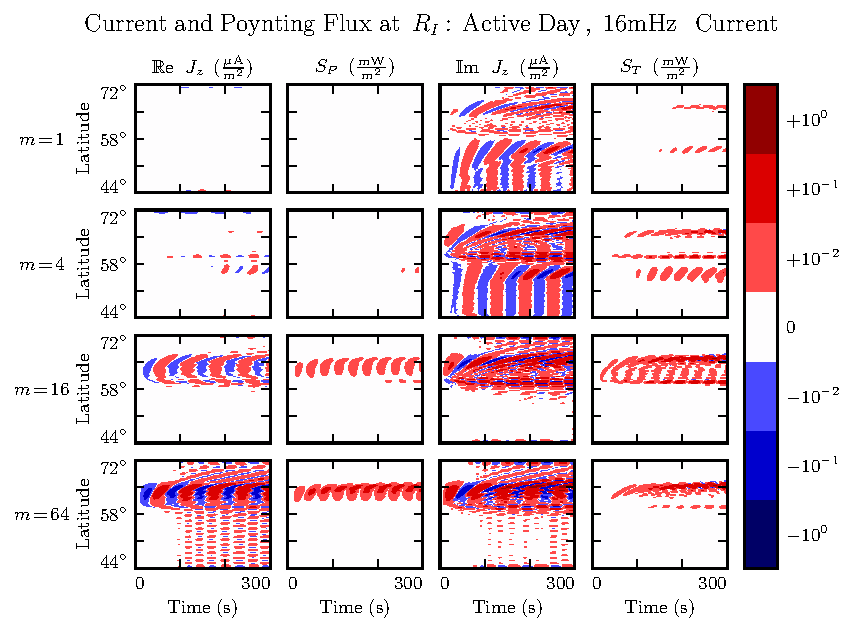
\includegraphics[width=\textwidth]{figures/current_poynting_flux.pdf}
    \caption[Current and Poynting Flux at the Ionosphere]{
      Perhaps unsurprisingly, field-aligned current structures at the ionospheric boundary line up with Poynting flux structures. The imaginary component of the current lines up with the toroidal Poynting flux (which is the product of imaginary $E_x$ and imaginary $B_y$), while the real current lines up with the poloidal Poynting flux ($E_y$ and $B_x$ are real). 
    }
    \label{fig_current_poynting_flux}
\end{figure}




\begin{figure}[!htb]
    \centering
    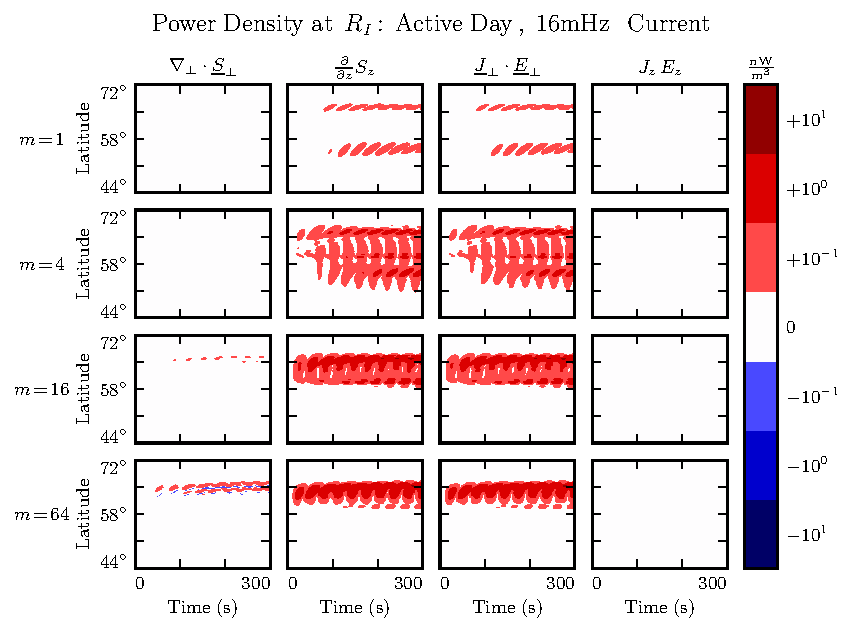
\includegraphics[width=\textwidth]{figures/power_density.pdf}
    \caption[Power Density at the Ionosphere]{
      While field-aligned currents can be of significant size, they are not particularly good at depositing energy in the ionosphere. Energy deposited by the Poynting flux matches closely with Joule dissipation from the perpendicular currents -- energy conservation! -- while $J_\parallel E_\parallel$ is smaller by several orders of magnitude. 
    }
    \label{fig_power_density}
\end{figure}



% -----------------------------------------------------------------------------
% -----------------------------------------------------------------------------
% -----------------------------------------------------------------------------
\subsection{Inertial Length Scales}
  \label{sec_lengths}


\begin{figure}[!htb]
    \centering
    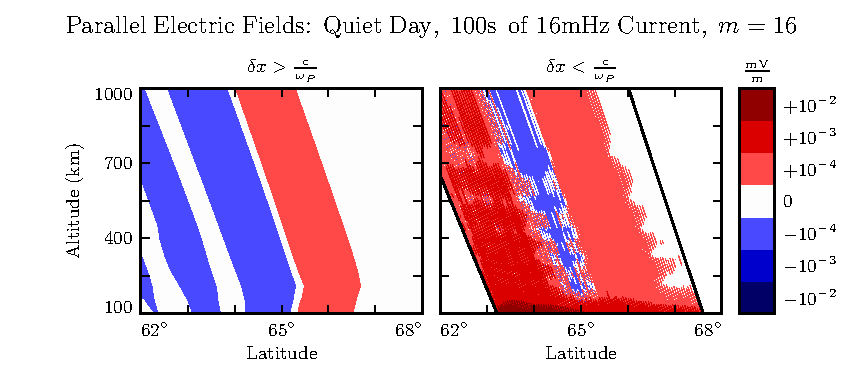
\includegraphics[width=\textwidth]{figures/inertial_length.pdf}
    \caption[Parallel Electric Fields by Perpendicular Grid Resolution]{
      The parallel electric field develops significant structure when the perpendicular grid resolution is smaller than the electron inertial length. Unfortunately, such runs are prohibitively expensive. The lower panel -- which still fails to resolve wave structure properly -- represents a 100-fold increase in computational time. 
    }
    \label{fig_inertial_length}
\end{figure}




\todo{We do a few runs which sorta resolve the electron inertial length. It's about \SI{2}{\km}, and we get resolution down to \SI{0.7}{\km}. This is a factor of ten increase in resolution, and an additional factor of ten decrease in the time step (due to the drop in \Alfven crossing time). It's not enough. FIG is clearly not well-resolved. Those wigglies are probably about to cause a crash. }



test reference: \cref{fig_inertial_length} \cref{fig_power_density}

\todo{Note, again, that only the figures in the present chapter include electron inertia. Those in \cref{ch_results,ch_rbsp} do not, for the sake of stability and computational cost. }


With a bit of algebra, the meridional components of the dispersion tensor from \cref{sec_high_alt} provide a comparison of the parallel and perpendicular electric field magnitudes.
\begin{align}
  \frac{E_\parallel}{E_\bot} &= \frac{- k_\parallel k_\bot c^2 }{ \omega^2 - k_\bot^2 c^2 - \op^2 } \sim \frac{k^2 c^2 }{\op^2}
\end{align}


% -----------------------------------------------------------------------------
% -----------------------------------------------------------------------------
% -----------------------------------------------------------------------------
\subsection{Field-Aligned Current}
  \label{sec_fac}

\todo{The field-aligned current activity lines up with the Poynting flux. Poloidal Poynting flux is calculated from real $E_y$ and $B_x$. Toroidal Poynting flux is imaginary $E_x$ and $B_y$. The real component of the field-aligned current matches up with the poloidal, and the imaginary component lines up with the toroidal. }

\todo{Over the bulk of the simulation, each field is overwhelmingly either real or imaginary. However, that gets muddled at the ionosphere by the Hall conductivity (rather than being purely a function of azimuthal derivatives). }


\todo{Notably, while the net Poynting flux is downward almost everywhere, field-aligned currents alternate between upward and downward flow. Perhaps this has to do with Poynting flux being a quadratic quantity while current is linear? }

The ``wigglies'' visible in the lower-left corner of \cref{fig_current_poynting_flux} suggests overcorrection due to an improperly-coarse grid. See \cref{sec_lengths}. 

\todo{Field-aligned currents can be of significant size, but they're not particularly good at depositing energy in the ionosphere. As would be expected from energy conservation, $\nabla \cdot \vec{S}$ closely resembles $\vec{J} \cdot \vec{E}$, but only a vanishingly small portion of that is due to $J_z E_z$. }

\todo{Are we really computing the electric fields faithfully? As touched on in \cref{sec_inertia_fields}, the perpendicular wavelength is important for determining the strength of the parallel electric field. This is because everything depends on derivatives, not magnitudes. }


The electron inertial length $\frac{c}{\op}$ is on the order of \SI{1}{\km}, smaller than the wavelength of a field line resonance by three or four orders of magnitude. That is, at high altitude, the parallel electric field is expected to be smaller than the perpendicular electric field by a factor of \num{e7} -- perhaps more, depending on how closely the wave vector is aligned to the magnetic field. That seems fine -- note that \cref{fig_electric_field_snapshots} shows that max $E_\parallel$ is 4 to 5 orders larger than max $E_\bot$... plus high altitude is the parallel field's minimum and the perpendicular field's maximum. 




\todo{A typical run has maximum perpendicular electric field on the order of \SI{10}{\mV/\meter}. Maybe a bit more. Field structures vary on the order of as little as $\sim\SI{1}{\degree}$. That could give up to $\curl{E} \sim \SI{e2}{nT/\second}$. In comparison parallel electric fields max out around \SI{e-3}{\mV/\meter}. If that varies as a scale of the inertial length -- as we expect, recalling \cref{sec_boris} -- that's order of \SI{1}{\km}, it could give $\curl{E} \sim \SI{1}{nT/\second}$. Plausibly large enough to have a visible effect. Note that the electron inertial length only needs to be resolved in the perpendicular direction, since that's where we're taking curls of the parallel electric field... which is the only quantity expected to change significantly (to lowest order) as a result of electron inertial effects. }

\todo{This poses a significant computational cost. Within the plasmasphere, the inertial length is on the order of \SI{0.1}{\km}. That's two-plus orders of magnitude smaller than the present grid. Moving the inner boundary from $L=2$ to $L=5$ makes up half of that. }


\todo{The moral of the present section is that proper handling of electron inertial effects will probably show additional structure at small scales... but that simulating those structures is computationally expensive in terms of computational expense, even in 2.5D. }


